

\section{Implementation}
\label{sec:implementation}

We implemented our approach in a publicly available end-to-end tool~\cite{ArtifactRepository}. Our tool consists in over $20{,}000$ LoC written in \texttt{Rust}.
%
We next elaborate on the architecture of our tool and the various optimizations we added to allow it to run efficiently.

%The implementation..

%\begin{enumerate}
%	\item The extra things we did to make the thing actually run
%	\item Code architecture
%	\item Optimizations
%\end{enumerate}



\subsection{Code Architecture}

\label{subsec:codeArchitecture}

Our tool implements an end-to-end serializability checker for arbitrary inputs programs. If the program is serializable, we return a proof thereof; otherwise, if it is not serializable --- a counterexample is given to the user, for an interleaving that can result to request/response pairs that are unattainable in any serial execution.
%
Our workflow translates the decidability problem to an equivalent Petri Net reachability question (for unbounded nets). in which (i) the Petri Net represents all possible interleavings of the problem; and (ii) the reachability query represents a semilinear set (equivalently, a Presburger arithmetic encoding) of all (request,response) pairs that cannot be attained in any serial execution.
%
As Petri Net reachability is Ackermann complete~\cite{CzWo22}, we added various optimizations to expedite the search process, both in the Petri Net level and the property encoding level.
%
The pipeline of our approach is depicted in Fig.~\ref{fig:full_program_flow}, and includes the following:
 

\begin{enumerate}
	\item \textbf{Input \& Parsing.} Our model receives one of two textual representation of the program in question: (i) a \texttt{ser} program with the syntax described in Sec.~\ref{sec:problem-definition} or (ii) a \texttt{JSON} file which directly encodes the transitions of our networking system (NS). In the case of the former, an additional step takes place, in which the input program is parsed (using the \texttt{parser.rs} module) to an expression tree and then translated to an equivalent networking system. The NS is represented as a struct in the \texttt{ns.rs} module. 
	
	\item \textbf{Petri Net Conversion.} The NS is then translated into a Petri Net (see the \texttt{petri.rs} module) which represents the interleavings of the NS. Each place represents a local state or a global state, and each token represents a single in-flight request or a terminated response. The PN is encoded in the de-facto standard \texttt{.net} encoding, in order to be compatible with off-the-shelf PN model checkers. 
	
	\item \textbf{Semilinear Conversion.} 
	This includes a set of modules (\texttt{kleene.rs}, \texttt{semilinear.rs}, and \texttt{presburger.rs}) which generate a smeilinear set encoding of the non serializable outputs. This conversion is done by the following pipeline: (1) the NS is translated to an NFA encoding all possible request/response pairs of the input program; (2) This NFA is translated to a regex (via Kleene's Theorem) and then project (via the Parikh Image) to a semilinear set. The (finite) encoding of the semilinear set symbolically represents all outputs attained via serializable executions of the program, running for an unbounded number of steps; (3) finally, we complement the semilinear set to attain a semilinear set encoding all outputs unattainable via serial executions. At the end of the pipeline, an \texttt{XML}-formatted output encodes a reachability query which encapsulates constraints over the PN token count.
	
	
	\item \textbf{Reachability Engine.} The PN and the reachability query are fed to a state-of-the-art PN model checker, which runs \textit{Bounded Model Checking} (BMC)~\cite{BiCiClZh99} in search of a counterexample; and \textit{state equation reasoning}~\cite{Mu77} in order to prove non-reachability. This engine is implemented in the \texttt{reachability.rs} and \texttt{reachability\_with\_proofs.rs}  modules.
	%
	In order to expedite the reachability search, the we replace the single ``large'' PN and query with multiple smaller PNs, each coupled with a sub-query encoding a separate disjunct from the original query.
	We iteratively solve the disjuncts on the fly, until reaching \sat, in which case, we have a counterexample; otherwise, if a disjunct is \unsat, we continue to the next one. If all disjuncts are \unsat, we render the original program as serializable.
	
	
	\item \textbf{Proof \& Certificate Handling.} If the query is \texttt{SAT}, we reconstruct a non-serializable NS-level execution and validates its correctness. Otherwise, if all disjuncts are \texttt{UNSAT}, our proof module extracts a separate proof for each disjunct. We subsequently ``stich'' these proofs to a single inductive invariant of the full query, and project it to the NS-level, representing a full inductive proof certificate for serializability. Our checker also validates that the inductive invariant is correct, i.e., (i) includes the initial state of the system; (ii) is inductive with regard to the transitions; and (iii) implies that the reachability query is \texttt{UNSAT}, and hence implying serializability. 
	
	
	\item \textbf{Instrumentation \& Logging.} Throughout the pipeline, the input size and performance metrics (number of places, transitions, constraint complexity, timings) are recorded. The logger outputs structured \texttt{CSV} and \texttt{JSON} logs for later analysis. 
	%
	We also assemble an \texttt{HTML} report which embeds the original net, symbolic constraints, reachability results, proof outlines, and profiling graphs.
%	\item \textbf{Debug Report Generation.} Finally, a human-readable \texttt{HTML} report is assembled: it embeds the original net, symbolic constraints, reachability results, proof outlines, and profiling graphs. This interactive report allows users to drill down into each transition firing, constraint check, and proof obligation.
	
%	\item \textbf{Output Delivery.} The crate exposes a simple CLI and library API. Users obtain either a Boolean reachability verdict (with optional certificate), raw log files, or a full HTML debug report, depending on invocation flags.
	
	\item \textbf{Optimizations.} As we extensively elaborate later, we also include multiple optimizations, both re represent the semilinear sets succinctly, and to prune the PN. These optimizations significantly reduce the search space and expedite the model checking process.
\end{enumerate}



%\noindent
%This linear pipeline - \emph{parse} -> \emph{model} -> \emph{normalize} -> \emph{analyze} -> \emph{prove} -> \emph{report} --- ensures a clear separation of concerns, easy extensibility (e.g., swapping backends), and comprehensive traceability from input to certified result.```


\begin{figure}[!htbp]
	\centering
	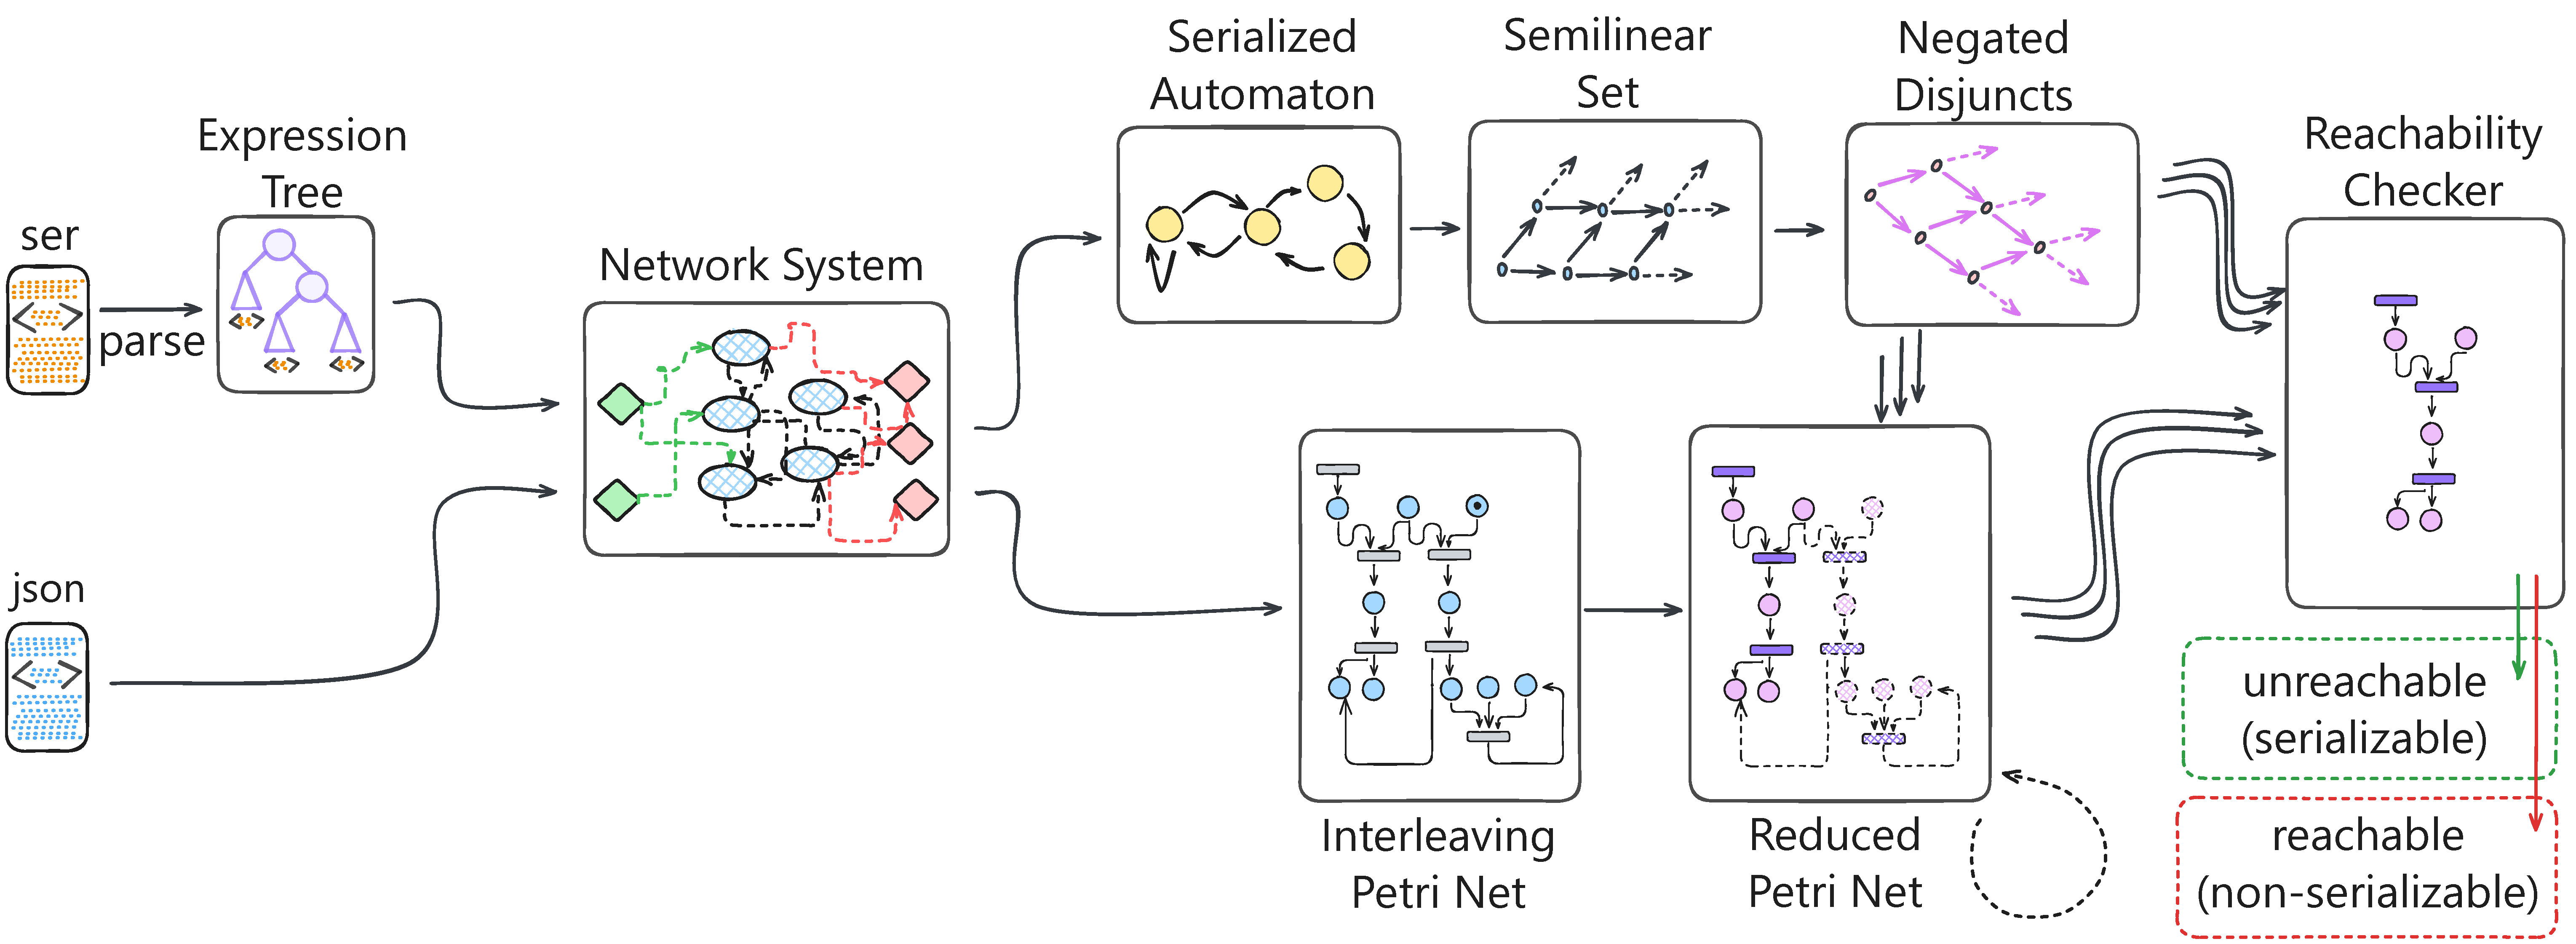
\includegraphics[width=1.0\textwidth]{plots/full_program_flow.pdf}
	\caption{Full program flow. If the program is unreachable --- a serializability proof is produced; otherwise, if it is reachable --- a counterexample trace is generated.
	For simplicity, we omit the backward arrows translating invariants (if serializable) or counterexample traces (if non) back to the NS level.}
	\label{fig:full_program_flow}
\end{figure}


\subsection{Optimizations}

\paragraph{Bidirectional Pruning of the Petri Net}
Before any heavy symbolic reasoning takes place, we apply bidirectional pruning on the underlying PN.  In the forward pass, we traverse from the initial marking to identify all places and transitions that could ever fire; in the backward pass, we traverse backward from any place that can influence a target constraint, and identify transitions and places that cannot contribute to reaching it.  By iteratively repeating forward passes and backward passes until convergence, we remove every component of the net that cannot both originate and contribute to the reachable target set.  This dramatically shrinks the net in practice, often converting an intractably large model into one small enough for exhaustive analysis.
%
We depict this in Fig.~\ref{fig:bidirectional_pruning}, and give a formal proof of correctness in Appendix~\ref{appendix:BidirectionalProof}.

\paragraph{Redundant‐Constraint Elimination}
When manipulating Presburger sets or their semilinear representations, it is common for some inequalities or disjuncts to add no new coverage beyond what other constraints already guarantee.  The redundant‐constraint elimination pass inspects each linear inequality and each disjunct in a disjunctive normal form, testing whether it is implied by the rest.  Any constraint or disjunct found redundant is dropped, ensuring that subsequent intersection, union, and projection operations work on the smallest necessary formula.  This streamlines the logic formula and prevents exponential blow‐up of case distinctions during solver invocations.
%
%Every time you build or star a semilinear set, you prune out any “period” vectors that are rendered useless by earlier steps:. nce you’ve accumulated a bunch of LinearSet components, you try to merge any that mathematically subsume one another:

\paragraph{Generating Fewer Constraints}
During set‐construction--- especially when introducing new existentially‐quantified variables or combining transition effects, we selectively avoid generating any marking that would strictly dominate an already‐seen solution.  In effect, whenever a candidate disjunct would yield a superset of an existing one, it is skipped entirely.  This ``generate‐less” heuristic stops the proliferation of large, overlapping regions in the semilinear description, trading off completeness of intermediate case‐enumeration for concise final representations.  In benchmarks with large state‐spaces, it can reduce the number of intermediate branches by orders of magnitude.

%in both the Regex and SemilinearSet Kleene-algebra instances. Concretely, instead of always building the full new structure and pruning it later, operations like union (plus) and concatenation (times) do a quick check for trivial cases and drop “zero” or “one” elements on the spo

\paragraph{Executing Kleene Elimination in a Strategic Order:}
When converting an NFA to a single regex, we pick the next state to eliminate by heuristically choosing the  state with the fewest incoming and outgoing edges.
This optimization allows circumventing 
overblown expressions resulting in naive translations, especially with regard to  Kleene closures (the “\(\mathsf{*}\)” operator).  Instead, we analyze the structure of sub-expressions under the various operators --- estimating their branching factor, and reorder them so that simpler, low‐branching components are expanded first.  This adaptive ordering often leads to early detection of fixed points or dead‐ends, preventing the combinatorial explosion that arises when complex loops are expanded prematurely.  




\begin{figure}[!htbp]
	\centering
	
	% Top row: (a), (b)
	\begin{subfigure}[b]{0.45\textwidth}
		\centering
		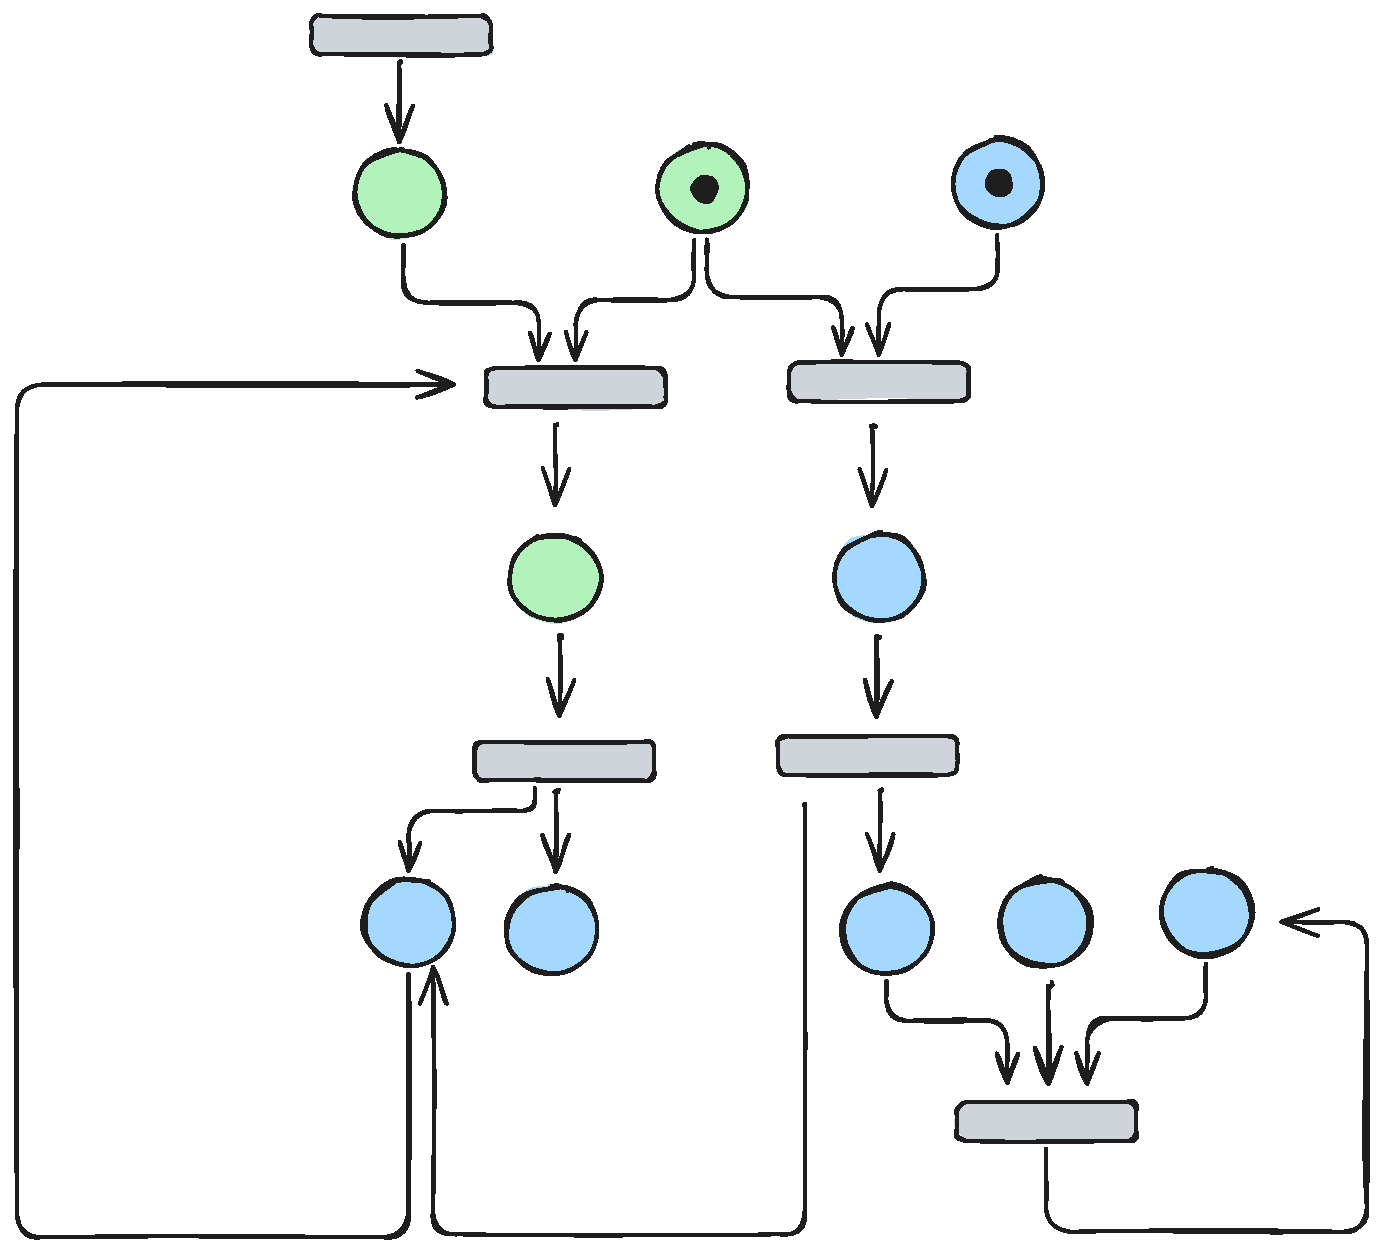
\includegraphics[width=\textwidth]{plots/bidirectional_pruning_step_a_updated.pdf}
		\caption{Step 0: initial petri net, before pruning.}
		\label{fig:step:a}
	\end{subfigure}\hfill
	\begin{subfigure}[b]{0.45\textwidth}
		\centering
		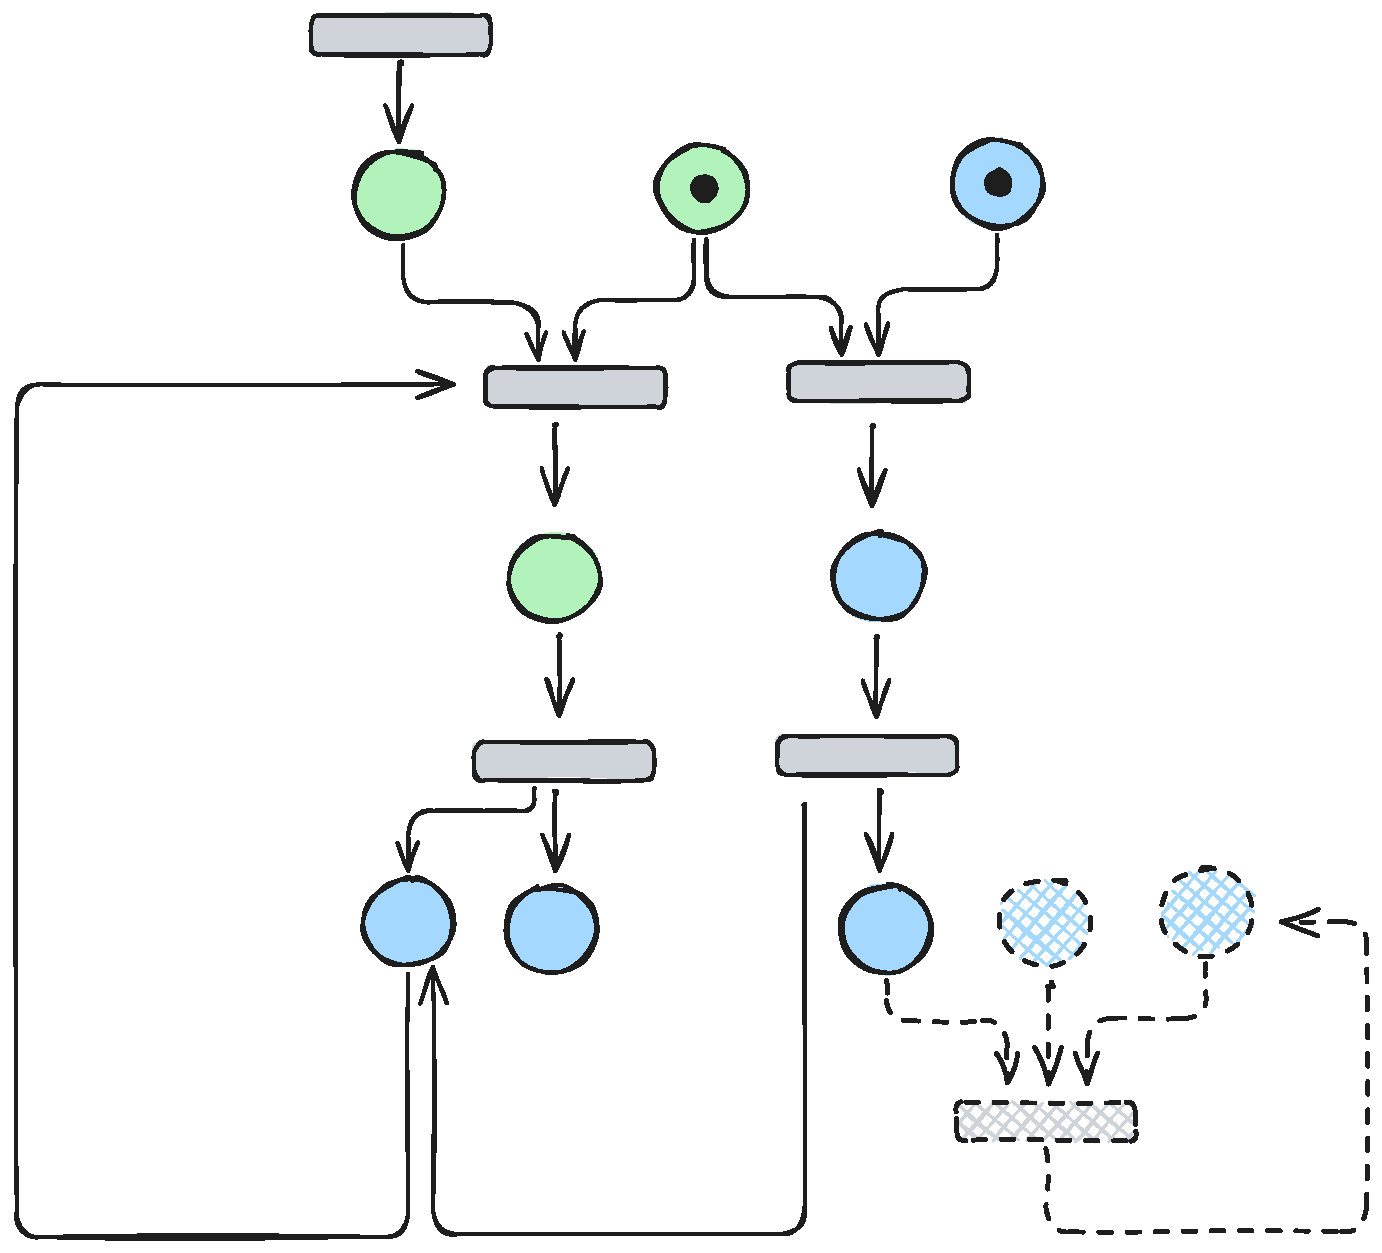
\includegraphics[width=\textwidth]{plots/bidirectional_pruning_step_b_updated.pdf}
		\caption{Step 1: first forward pass.}
		\label{fig:step:b}
	\end{subfigure}
	
	\vspace{1em}
	
	% Bottom row: (c), (d), and (e) matching (d)’s height
	\begin{subfigure}[b]{0.30\textwidth}
		\centering
		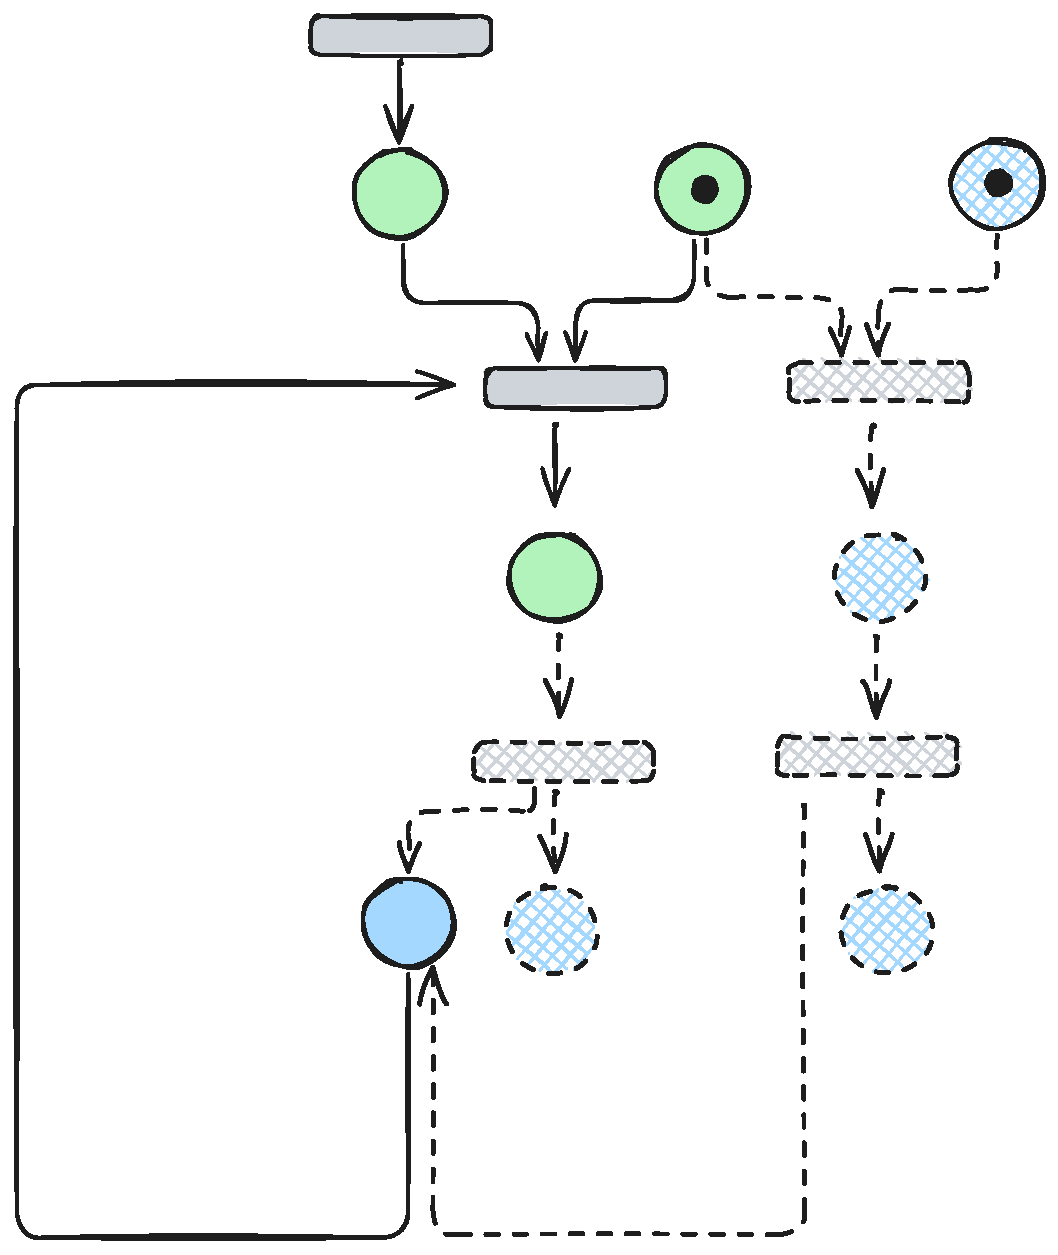
\includegraphics[width=\textwidth]{plots/bidirectional_pruning_step_c_updated.pdf}
		\caption{Step 3: first backward pass.}
		\label{fig:step:c}
	\end{subfigure}\hfill
	\begin{subfigure}[b]{0.23\textwidth}
		\centering
		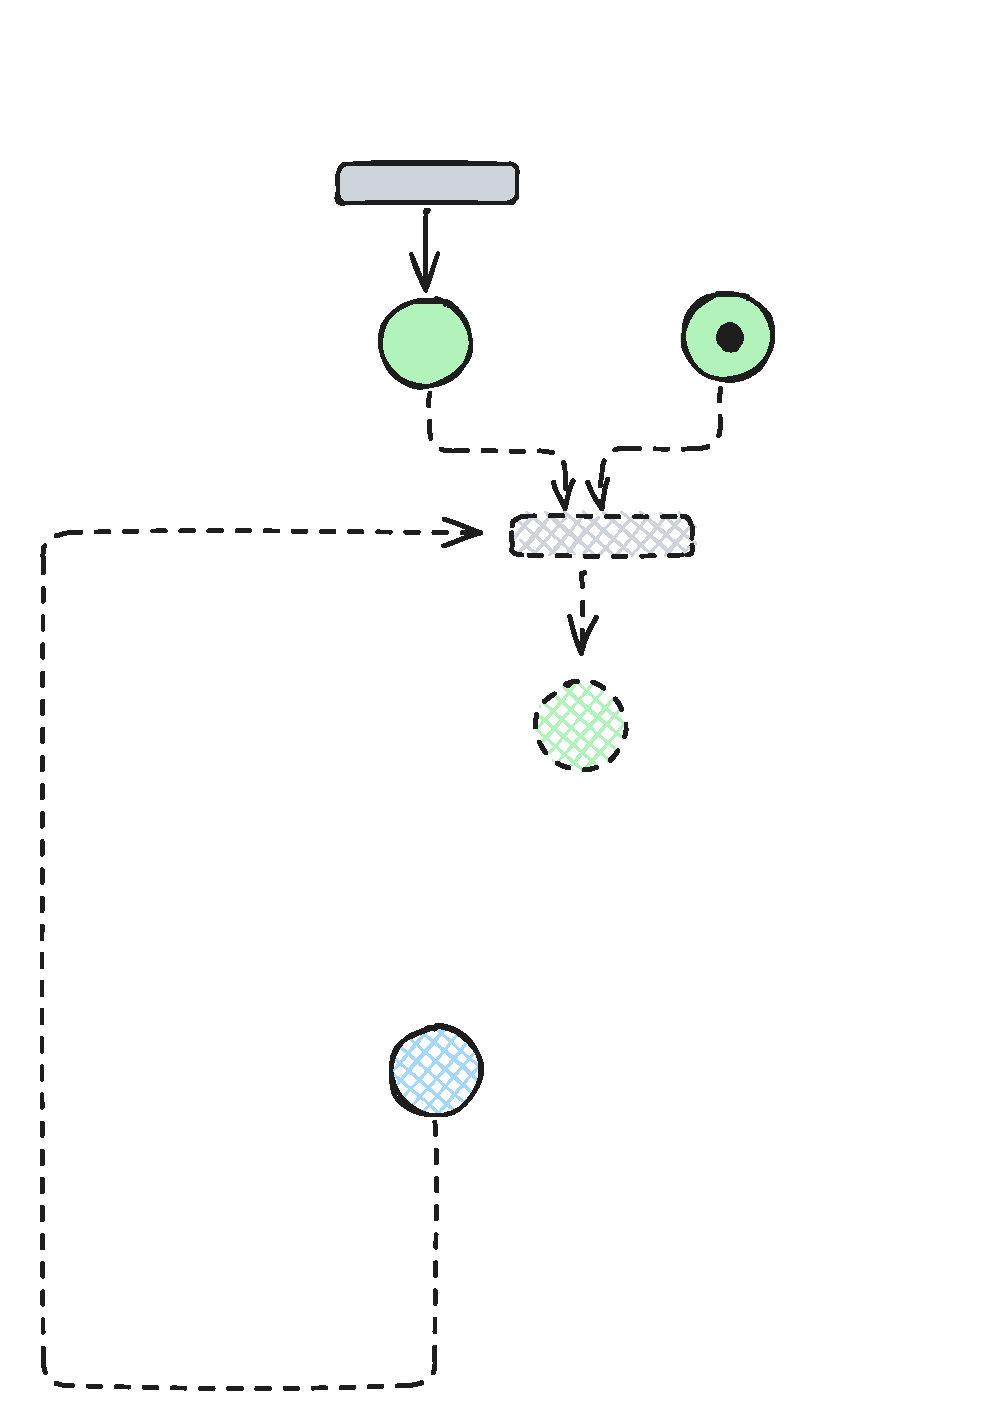
\includegraphics[width=\textwidth]{plots/bidirectional_pruning_step_d_updated_2.pdf}
		\caption{Step 4: second forward pass.}
		\label{fig:step:d}
	\end{subfigure}\hfill
	% <-- three-arg form: [vpos][total height][inner vpos]
	\begin{subfigure}[b][\subfigheight][b]{0.23\textwidth}
		\centering
		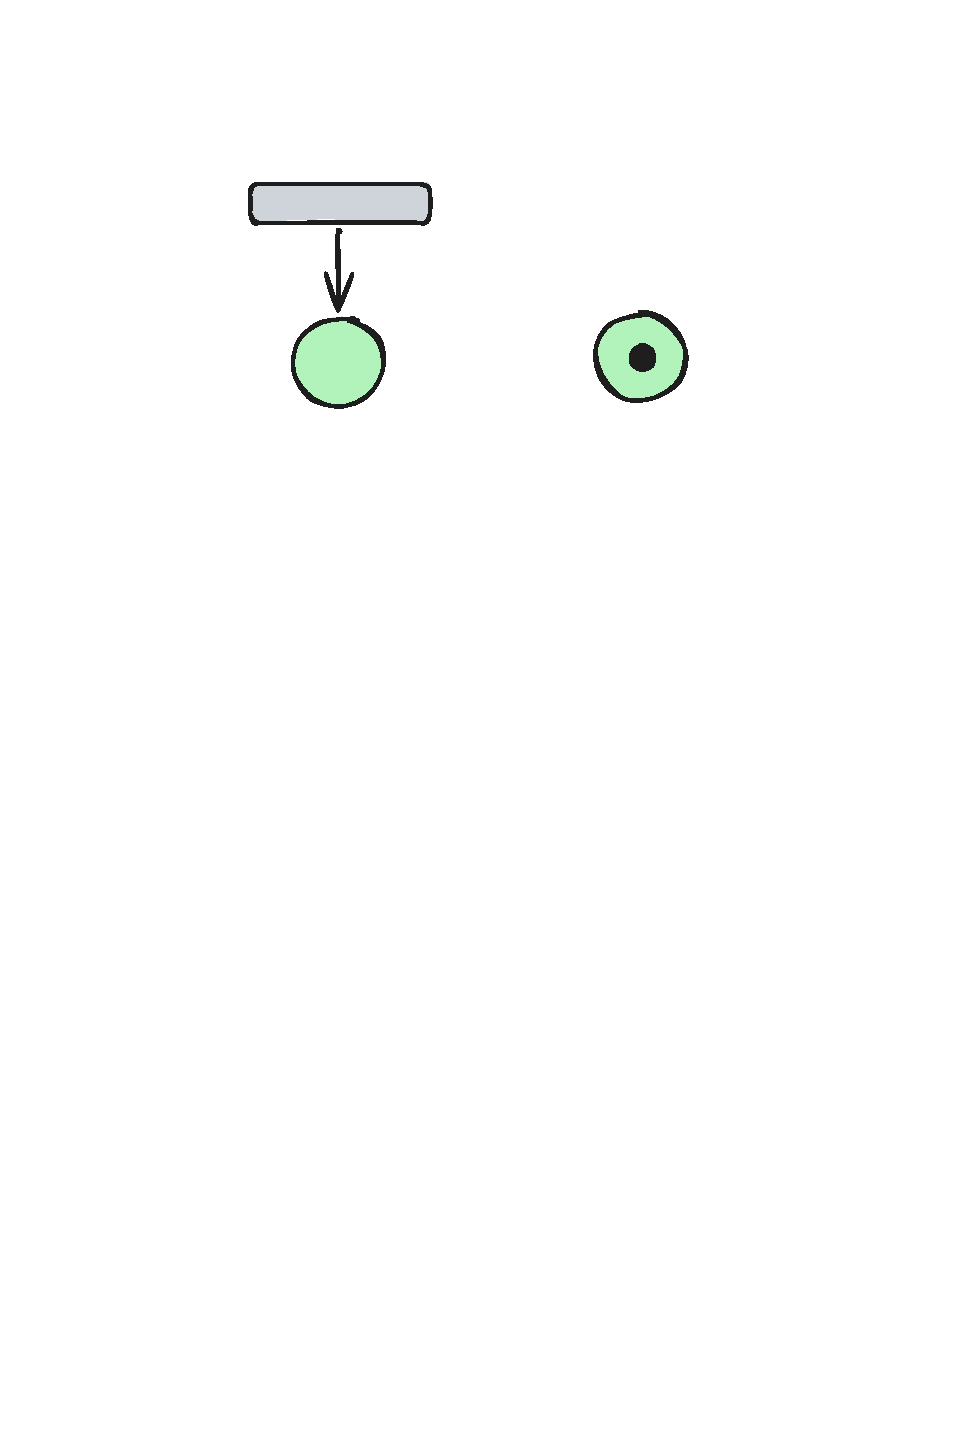
\includegraphics[width=\textwidth]{plots/bidirectional_pruning_step_e_updated_2.pdf}
		\caption{Step 6: final petri net.}
		\label{fig:step:e}
	\end{subfigure}
	
	\caption{A Petri Net after four iterations of bidirectional pruning: two forward passes and two backward passes. Black dots represent initial token markings; green places represent places that are allowed to be reachable in our constraints (i.e., aren't fixed to zero tokens in the final marking). Dashed shapes represent places and transitions that are identified as removable in the current iteration, and will be removed after it ends.}
	\label{fig:bidirectional_pruning}
\end{figure}




%\newpage